\batchmode
\documentclass[12pt,leqno,]{article}
\RequirePackage{ifthen}


\usepackage{boxedminipage}


\usepackage{html}


%
\renewcommand{\bbm}{\vspace{5pt}

\noindent\begin{boxedminipage}{2.0\linewidth}} 


\usepackage{graphicx}
\usepackage{hyperref}
\usepackage{verbatim}
\usepackage[cmbase]{flexisym}
\usepackage{bbold}


\usepackage{breqn}
\setkeys{breqn}{compact}


\usepackage{makeidx} 
\makeindex

%
\providecommand{\ebm}{\end{boxedminipage}\vspace{5pt}

\noindent} 

\setlength{\fboxrule}{0.1pt}  

\setlength{\fboxsep}{10pt} 



\setlength{\textwidth}{180mm} 

\setlength{\oddsidemargin}{15mm} 

\addtolength{\oddsidemargin}{-1in} 

\setlength{\evensidemargin}{15mm} 

\addtolength{\evensidemargin}{-1in} 

%
\providecommand{\ifrac}[2]{\frac{#1}{#2}}%
\providecommand{\ifracd}[2]{\frac{#1}{#2}}%
\providecommand{\ifracn}[2]{\frac{#1}{#2}}%
\providecommand{\isubscript}[2]{{#1}_{#2}}%
\providecommand{\iexpt}[2]{{#1}^{#2}}%
\providecommand{\isqrt}[1]{\sqrt{#1}} 

%
\providecommand{\ket}[1]{{\lvert#1 \rangle}}%
\providecommand{\bra}[1]{{\langle#1 \rvert}}%
\providecommand{\func}[2]{{\bf #1}($#2$)}%
\providecommand{\marray}[2]{{\bf #1}[$#2$]}%
\providecommand{\fs}[1]{{\bf #1}} 

%
\providecommand{\ifs}[1]{{\bf #1}\index{#1@{\bf #1}}}  % bold index entry plus bold in text%
\providecommand{\ibd}[1]{\index{#1@{\bf #1}}}  % bold index entry%
\providecommand{\iit}[1]{\index{#1@{\it #1}}}  % italic index entry%
\providecommand{\ipname}[1]{{\it #1}\index{#1@{\it #1}}}%
\providecommand{\pname}[1]{{\it #1}}  % software name%
\providecommand{\imarray}[2]{{\bf #1}[$#2$]\index{#1@{{\bf #1}[$#2$]}}}  % \marray with index entry%
\providecommand{\ifunc}[2]{{\bf #1}($#2$)\index{#1@{\bf #1}($#2$)}}  % \func with index entry%
\providecommand{\qinf}{ {\it qinf } }  % the name of this package%
\providecommand{\qinfp}{{\it qinf}}  % use at end of sentece for period

%
\providecommand{\farg}[1]{{\it #1}}  % an argument

%
\providecommand{\maxcom}{\textsuperscript{$\dagger$}} 




\usepackage[dvips]{color}


\pagecolor{white}

\usepackage[]{inputenc}



\makeatletter

\makeatletter
\count@=\the\catcode`\_ \catcode`\_=8 
\newenvironment{tex2html_wrap}{}{}%
\catcode`\<=12\catcode`\_=\count@
\newcommand{\providedcommand}[1]{\expandafter\providecommand\csname #1\endcsname}%
\newcommand{\renewedcommand}[1]{\expandafter\providecommand\csname #1\endcsname{}%
  \expandafter\renewcommand\csname #1\endcsname}%
\newcommand{\newedenvironment}[1]{\newenvironment{#1}{}{}\renewenvironment{#1}}%
\let\newedcommand\renewedcommand
\let\renewedenvironment\newedenvironment
\makeatother
\let\mathon=$
\let\mathoff=$
\ifx\AtBeginDocument\undefined \newcommand{\AtBeginDocument}[1]{}\fi
\newbox\sizebox
\setlength{\hoffset}{0pt}\setlength{\voffset}{0pt}
\addtolength{\textheight}{\footskip}\setlength{\footskip}{0pt}
\addtolength{\textheight}{\topmargin}\setlength{\topmargin}{0pt}
\addtolength{\textheight}{\headheight}\setlength{\headheight}{0pt}
\addtolength{\textheight}{\headsep}\setlength{\headsep}{0pt}
\setlength{\textwidth}{349pt}
\newwrite\lthtmlwrite
\makeatletter
\let\realnormalsize=\normalsize
\global\topskip=2sp
\def\preveqno{}\let\real@float=\@float \let\realend@float=\end@float
\def\@float{\let\@savefreelist\@freelist\real@float}
\def\liih@math{\ifmmode$\else\bad@math\fi}
\def\end@float{\realend@float\global\let\@freelist\@savefreelist}
\let\real@dbflt=\@dbflt \let\end@dblfloat=\end@float
\let\@largefloatcheck=\relax
\let\if@boxedmulticols=\iftrue
\def\@dbflt{\let\@savefreelist\@freelist\real@dbflt}
\def\adjustnormalsize{\def\normalsize{\mathsurround=0pt \realnormalsize
 \parindent=0pt\abovedisplayskip=0pt\belowdisplayskip=0pt}%
 \def\phantompar{\csname par\endcsname}\normalsize}%
\def\lthtmltypeout#1{{\let\protect\string \immediate\write\lthtmlwrite{#1}}}%
\newcommand\lthtmlhboxmathA{\adjustnormalsize\setbox\sizebox=\hbox\bgroup\kern.05em }%
\newcommand\lthtmlhboxmathB{\adjustnormalsize\setbox\sizebox=\hbox to\hsize\bgroup\hfill }%
\newcommand\lthtmlvboxmathA{\adjustnormalsize\setbox\sizebox=\vbox\bgroup %
 \let\ifinner=\iffalse \let\)\liih@math }%
\newcommand\lthtmlboxmathZ{\@next\next\@currlist{}{\def\next{\voidb@x}}%
 \expandafter\box\next\egroup}%
\newcommand\lthtmlmathtype[1]{\gdef\lthtmlmathenv{#1}}%
\newcommand\lthtmllogmath{\dimen0\ht\sizebox \advance\dimen0\dp\sizebox
  \ifdim\dimen0>.95\vsize
   \lthtmltypeout{%
*** image for \lthtmlmathenv\space is too tall at \the\dimen0, reducing to .95 vsize ***}%
   \ht\sizebox.95\vsize \dp\sizebox\z@ \fi
  \lthtmltypeout{l2hSize %
:\lthtmlmathenv:\the\ht\sizebox::\the\dp\sizebox::\the\wd\sizebox.\preveqno}}%
\newcommand\lthtmlfigureA[1]{\let\@savefreelist\@freelist
       \lthtmlmathtype{#1}\lthtmlvboxmathA}%
\newcommand\lthtmlpictureA{\bgroup\catcode`\_=8 \lthtmlpictureB}%
\newcommand\lthtmlpictureB[1]{\lthtmlmathtype{#1}\egroup
       \let\@savefreelist\@freelist \lthtmlhboxmathB}%
\newcommand\lthtmlpictureZ[1]{\hfill\lthtmlfigureZ}%
\newcommand\lthtmlfigureZ{\lthtmlboxmathZ\lthtmllogmath\copy\sizebox
       \global\let\@freelist\@savefreelist}%
\newcommand\lthtmldisplayA{\bgroup\catcode`\_=8 \lthtmldisplayAi}%
\newcommand\lthtmldisplayAi[1]{\lthtmlmathtype{#1}\egroup\lthtmlvboxmathA}%
\newcommand\lthtmldisplayB[1]{\edef\preveqno{(\theequation)}%
  \lthtmldisplayA{#1}\let\@eqnnum\relax}%
\newcommand\lthtmldisplayZ{\lthtmlboxmathZ\lthtmllogmath\lthtmlsetmath}%
\newcommand\lthtmlinlinemathA{\bgroup\catcode`\_=8 \lthtmlinlinemathB}
\newcommand\lthtmlinlinemathB[1]{\lthtmlmathtype{#1}\egroup\lthtmlhboxmathA
  \vrule height1.5ex width0pt }%
\newcommand\lthtmlinlineA{\bgroup\catcode`\_=8 \lthtmlinlineB}%
\newcommand\lthtmlinlineB[1]{\lthtmlmathtype{#1}\egroup\lthtmlhboxmathA}%
\newcommand\lthtmlinlineZ{\egroup\expandafter\ifdim\dp\sizebox>0pt %
  \expandafter\centerinlinemath\fi\lthtmllogmath\lthtmlsetinline}
\newcommand\lthtmlinlinemathZ{\egroup\expandafter\ifdim\dp\sizebox>0pt %
  \expandafter\centerinlinemath\fi\lthtmllogmath\lthtmlsetmath}
\newcommand\lthtmlindisplaymathZ{\egroup %
  \centerinlinemath\lthtmllogmath\lthtmlsetmath}
\def\lthtmlsetinline{\hbox{\vrule width.1em \vtop{\vbox{%
  \kern.1em\copy\sizebox}\ifdim\dp\sizebox>0pt\kern.1em\else\kern.3pt\fi
  \ifdim\hsize>\wd\sizebox \hrule depth1pt\fi}}}
\def\lthtmlsetmath{\hbox{\vrule width.1em\kern-.05em\vtop{\vbox{%
  \kern.1em\kern0.9 pt\hbox{\hglue.17em\copy\sizebox\hglue0.9 pt}}\kern.3pt%
  \ifdim\dp\sizebox>0pt\kern.1em\fi \kern0.9 pt%
  \ifdim\hsize>\wd\sizebox \hrule depth1pt\fi}}}
\def\centerinlinemath{%
  \dimen1=\ifdim\ht\sizebox<\dp\sizebox \dp\sizebox\else\ht\sizebox\fi
  \advance\dimen1by.5pt \vrule width0pt height\dimen1 depth\dimen1 
 \dp\sizebox=\dimen1\ht\sizebox=\dimen1\relax}

\def\lthtmlcheckvsize{\ifdim\ht\sizebox<\vsize 
  \ifdim\wd\sizebox<\hsize\expandafter\hfill\fi \expandafter\vfill
  \else\expandafter\vss\fi}%
\providecommand{\selectlanguage}[1]{}%
\makeatletter \tracingstats = 1 


\begin{document}
\pagestyle{empty}\thispagestyle{empty}\lthtmltypeout{}%
\lthtmltypeout{latex2htmlLength hsize=\the\hsize}\lthtmltypeout{}%
\lthtmltypeout{latex2htmlLength vsize=\the\vsize}\lthtmltypeout{}%
\lthtmltypeout{latex2htmlLength hoffset=\the\hoffset}\lthtmltypeout{}%
\lthtmltypeout{latex2htmlLength voffset=\the\voffset}\lthtmltypeout{}%
\lthtmltypeout{latex2htmlLength topmargin=\the\topmargin}\lthtmltypeout{}%
\lthtmltypeout{latex2htmlLength topskip=\the\topskip}\lthtmltypeout{}%
\lthtmltypeout{latex2htmlLength headheight=\the\headheight}\lthtmltypeout{}%
\lthtmltypeout{latex2htmlLength headsep=\the\headsep}\lthtmltypeout{}%
\lthtmltypeout{latex2htmlLength parskip=\the\parskip}\lthtmltypeout{}%
\lthtmltypeout{latex2htmlLength oddsidemargin=\the\oddsidemargin}\lthtmltypeout{}%
\makeatletter
\if@twoside\lthtmltypeout{latex2htmlLength evensidemargin=\the\evensidemargin}%
\else\lthtmltypeout{latex2htmlLength evensidemargin=\the\oddsidemargin}\fi%
\lthtmltypeout{}%
\makeatother
\setcounter{page}{1}
\onecolumn

% !!! IMAGES START HERE !!!

{\newpage\clearpage
\lthtmlinlinemathA{tex2html_wrap_inline3525}%
$i_1,\dots  ,i_n$%
\lthtmlinlinemathZ
\lthtmlcheckvsize\clearpage}

{\newpage\clearpage
\lthtmlinlinemathA{tex2html_wrap_inline3529}%
$.$%
\lthtmlinlinemathZ
\lthtmlcheckvsize\clearpage}

{\newpage\clearpage
\lthtmlinlinemathA{tex2html_wrap_inline3537}%
$\MathChar  "711B _x,\MathChar  "711B _y,\MathChar  "711B _z$%
\lthtmlinlinemathZ
\lthtmlcheckvsize\clearpage}

{\newpage\clearpage
\lthtmlinlinemathA{tex2html_wrap_inline3566}%
$j,i_1,\dots  ,i_m$%
\lthtmlinlinemathZ
\lthtmlcheckvsize\clearpage}

{\newpage\clearpage
\lthtmlinlinemathA{tex2html_wrap_inline3612}%
$a$%
\lthtmlinlinemathZ
\lthtmlcheckvsize\clearpage}

{\newpage\clearpage
\lthtmlinlinemathA{tex2html_wrap_inline3647}%
$i$%
\lthtmlinlinemathZ
\lthtmlcheckvsize\clearpage}

{\newpage\clearpage
\lthtmlinlinemathA{tex2html_wrap_inline3660}%
$\MathChar  "711A ,i_1,\dots  $%
\lthtmlinlinemathZ
\lthtmlcheckvsize\clearpage}

{\newpage\clearpage
\lthtmlinlinemathA{tex2html_wrap_inline3662}%
$\MathChar  "711A $%
\lthtmlinlinemathZ
\lthtmlcheckvsize\clearpage}

{\newpage\clearpage
\lthtmlinlinemathA{tex2html_wrap_inline3685}%
$n,\MathChar  "711A ,i_1,\dots  $%
\lthtmlinlinemathZ
\lthtmlcheckvsize\clearpage}

\stepcounter{section}
\stepcounter{subsection}
\stepcounter{section}
{\newpage\clearpage
\lthtmlfigureA{boxedminipage1208}%
\begin{boxedminipage}{2.0\linewidth}
\begin{verbatim}

(%i1) load("qinf.mac");
\end{verbatim}

\begin{dmath}[number={\%o1}]
 \verb|qinf.mac|\end{dmath}
\end{boxedminipage}%
\lthtmlfigureZ
\lthtmlcheckvsize\clearpage}

{\newpage\clearpage
\lthtmlinlinemathA{tex2html_wrap_inline1884}%
$A$%
\lthtmlinlinemathZ
\lthtmlcheckvsize\clearpage}

{\newpage\clearpage
\lthtmlinlinemathA{tex2html_wrap_inline1886}%
$m\times n$%
\lthtmlinlinemathZ
\lthtmlcheckvsize\clearpage}

{\newpage\clearpage
\lthtmlinlinemathA{tex2html_wrap_inline1888}%
$B$%
\lthtmlinlinemathZ
\lthtmlcheckvsize\clearpage}

{\newpage\clearpage
\lthtmlinlinemathA{tex2html_wrap_inline1890}%
$p\times q$%
\lthtmlinlinemathZ
\lthtmlcheckvsize\clearpage}

{\newpage\clearpage
\lthtmlinlinemathA{tex2html_wrap_inline1892}%
$n\times p$%
\lthtmlinlinemathZ
\lthtmlcheckvsize\clearpage}

{\newpage\clearpage
\lthtmlfigureA{boxedminipage1230}%
\begin{boxedminipage}{2.0\linewidth}
\begin{verbatim}

(%i1) 1 + 1;
\end{verbatim}

\begin{dmath}[number={\%o1}]
  2\end{dmath} 
\end{boxedminipage}%
\lthtmlfigureZ
\lthtmlcheckvsize\clearpage}

{\newpage\clearpage
\lthtmlinlinemathA{tex2html_wrap_inline1894}%
$a(x,y)$%
\lthtmlinlinemathZ
\lthtmlcheckvsize\clearpage}

{\newpage\clearpage
\lthtmlfigureA{boxedminipage1235}%
\begin{boxedminipage}{2.0\linewidth}
\begin{verbatim}

(%i2) a : 2 * 2;
\end{verbatim}

\begin{dmath}[number={\%o2}]
 4\end{dmath}
\begin{verbatim}

(%i3) a;
\end{verbatim}

\begin{dmath}[number={\%o3}]
 4\end{dmath}
\begin{verbatim}

(%i4) b : expand( (x+y)^4 );
\end{verbatim}

\begin{dmath}[number={\%o4}]
 y^{4}+4\*x\*y^{3}+6\*x^{2}\*y^{2}+4\*x^{3}\*y+x^{4}\end{dmath}
\end{boxedminipage}%
\lthtmlfigureZ
\lthtmlcheckvsize\clearpage}

{\newpage\clearpage
\lthtmlinlinemathA{tex2html_wrap_inline1896}%
$51$%
\lthtmlinlinemathZ
\lthtmlcheckvsize\clearpage}

{\newpage\clearpage
\lthtmlfigureA{boxedminipage1243}%
\begin{boxedminipage}{2.0\linewidth}
\begin{verbatim}

(%i5) b : expand( (x+y)^50 )$
(%i6) length(b);
\end{verbatim}

\begin{dmath}[number={\%o6}]
 51\end{dmath}
\end{boxedminipage}%
\lthtmlfigureZ
\lthtmlcheckvsize\clearpage}

{\newpage\clearpage
\lthtmlfigureA{boxedminipage1248}%
\begin{boxedminipage}{2.0\linewidth}
\begin{verbatim}

(%i7)  1  + sqrt(2);
\end{verbatim}

\begin{dmath}[number={\%o7}]
 \sqrt{2}+1\end{dmath}
\begin{verbatim}

index{floating point, conversion to}
(%i8)  1  + sqrt(2), float;
\end{verbatim}

\begin{dmath}[number={\%o8}]
 2.4142135623730949\end{dmath}
\end{boxedminipage}%
\lthtmlfigureZ
\lthtmlcheckvsize\clearpage}

{\newpage\clearpage
\lthtmlfigureA{boxedminipage1254}%
\begin{boxedminipage}{2.0\linewidth}
\begin{verbatim}

(%i9) f(x) := 3 * cos(x);
\end{verbatim}

\begin{dmath}[number={\%o9}]
 f\left(x\right):=3\*\cos x\end{dmath}
\begin{verbatim}

(%i10) f(a);
\end{verbatim}

\begin{dmath}[number={\%o10}]
 3\*\cos 4\end{dmath}
\begin{verbatim}

(%i11) f(0);
\end{verbatim}

\begin{dmath}[number={\%o11}]
 3\end{dmath}
\end{boxedminipage}%
\lthtmlfigureZ
\lthtmlcheckvsize\clearpage}

{\newpage\clearpage
\lthtmlinlinemathA{tex2html_wrap_inline1900}%
$i=\sqrt{-1}$%
\lthtmlinlinemathZ
\lthtmlcheckvsize\clearpage}

{\newpage\clearpage
\lthtmlfigureA{boxedminipage1259}%
\begin{boxedminipage}{2.0\linewidth}
\begin{verbatim}

(%i12) expand ( (1 + 2 * %i)^2 );
\end{verbatim}

\begin{dmath}[number={\%o12}]
 4\*i-3\end{dmath}
\end{boxedminipage}%
\lthtmlfigureZ
\lthtmlcheckvsize\clearpage}

{\newpage\clearpage
\lthtmlinlinemathA{tex2html_wrap_inline1902}%
$\pi$%
\lthtmlinlinemathZ
\lthtmlcheckvsize\clearpage}

{\newpage\clearpage
\lthtmlinlinemathA{tex2html_wrap_inline1904}%
$e$%
\lthtmlinlinemathZ
\lthtmlcheckvsize\clearpage}

{\newpage\clearpage
\lthtmlfigureA{boxedminipage1264}%
\begin{boxedminipage}{2.0\linewidth}
\begin{verbatim}

(%i13) cos(%pi/2);
\end{verbatim}

\begin{dmath}[number={\%o13}]
 0\end{dmath}
\begin{verbatim}

(%i14) %e^(%i * %pi/2);
\end{verbatim}

\begin{dmath}[number={\%o14}]
 i\end{dmath}
\end{boxedminipage}%
\lthtmlfigureZ
\lthtmlcheckvsize\clearpage}

\stepcounter{section}
{\newpage\clearpage
\lthtmlinlinemathA{tex2html_wrap_inline1906}%
$n \times 1$%
\lthtmlinlinemathZ
\lthtmlcheckvsize\clearpage}

{\newpage\clearpage
\lthtmlinlinemathA{tex2html_wrap_inline1908}%
$1
\times n$%
\lthtmlinlinemathZ
\lthtmlcheckvsize\clearpage}

{\newpage\clearpage
\lthtmlinlinemathA{tex2html_wrap_inline1910}%
$z$%
\lthtmlinlinemathZ
\lthtmlcheckvsize\clearpage}

\stepcounter{section}
\stepcounter{subsection}
{\newpage\clearpage
\lthtmlinlinemathA{tex2html_wrap_inline1912}%
$i_1,\ldots,i_n$%
\lthtmlinlinemathZ
\lthtmlcheckvsize\clearpage}

{\newpage\clearpage
\lthtmlinlinemathA{tex2html_wrap_inline1924}%
$\sigma_x,\sigma_y,\sigma_z$%
\lthtmlinlinemathZ
\lthtmlcheckvsize\clearpage}

{\newpage\clearpage
\lthtmlinlinemathA{tex2html_wrap_inline1926}%
$n$%
\lthtmlinlinemathZ
\lthtmlcheckvsize\clearpage}

{\newpage\clearpage
\lthtmlinlinemathA{tex2html_wrap_inline1928}%
$0$%
\lthtmlinlinemathZ
\lthtmlcheckvsize\clearpage}

{\newpage\clearpage
\lthtmlinlinemathA{tex2html_wrap_inline1930}%
$1$%
\lthtmlinlinemathZ
\lthtmlcheckvsize\clearpage}

{\newpage\clearpage
\lthtmlinlinemathA{tex2html_wrap_inline1932}%
$\sigma_z^{(1)} \otimes \cdots \otimes \sigma_z^{(n)}$%
\lthtmlinlinemathZ
\lthtmlcheckvsize\clearpage}

{\newpage\clearpage
\lthtmlinlinemathA{tex2html_wrap_inline1934}%
$i=0$%
\lthtmlinlinemathZ
\lthtmlcheckvsize\clearpage}

{\newpage\clearpage
\lthtmlinlinemathA{tex2html_wrap_inline1938}%
$i=1$%
\lthtmlinlinemathZ
\lthtmlcheckvsize\clearpage}

{\newpage\clearpage
\lthtmlinlinemathA{tex2html_wrap_inline1940}%
$-1$%
\lthtmlinlinemathZ
\lthtmlcheckvsize\clearpage}

{\newpage\clearpage
\lthtmlinlinemathA{tex2html_wrap_inline1942}%
${\lvert i_1,i_2,\ldots,i_n \rangle}.$%
\lthtmlinlinemathZ
\lthtmlcheckvsize\clearpage}

{\newpage\clearpage
\lthtmlfigureA{boxedminipage1286}%
\begin{boxedminipage}{2.0\linewidth}
\begin{verbatim}

(%i3) ketz(1)
\end{verbatim}

\begin{dmath}[number={\%o3}]
 \pmatrix{0\cr 1\cr }\end{dmath}
\end{boxedminipage}%
\lthtmlfigureZ
\lthtmlcheckvsize\clearpage}

{\newpage\clearpage
\lthtmlfigureA{boxedminipage1291}%
\begin{boxedminipage}{2.0\linewidth}
\begin{verbatim}

(%i4) braz(1)
\end{verbatim}

\begin{dmath}[number={\%o4}]
 \pmatrix{0&\linebreak[0]1\cr }\end{dmath}
\end{boxedminipage}%
\lthtmlfigureZ
\lthtmlcheckvsize\clearpage}

{\newpage\clearpage
\lthtmlfigureA{boxedminipage1296}%
\begin{boxedminipage}{2.0\linewidth}
\begin{verbatim}

(%i5) braz(0)
\end{verbatim}

\begin{dmath}[number={\%o5}]
 \pmatrix{1&\linebreak[0]0\cr }\end{dmath}
\end{boxedminipage}%
\lthtmlfigureZ
\lthtmlcheckvsize\clearpage}

{\newpage\clearpage
\lthtmlfigureA{boxedminipage1301}%
\begin{boxedminipage}{2.0\linewidth}
\begin{verbatim}

(%i6) braz(0,0)
\end{verbatim}

\begin{dmath}[number={\%o6}]
 \pmatrix{1&\linebreak[0]0&\linebreak[0]0&\linebreak[0]0\cr }\end{dmath}
\begin{verbatim}

(%i7) braz(1,1)
\end{verbatim}

\begin{dmath}[number={\%o7}]
 \pmatrix{0&\linebreak[0]0&\linebreak[0]0&\linebreak[0]1\cr }\end{dmath}
\begin{verbatim}

(%i8) alpha[1]*braz(1,1)+alpha[0]*braz(0,0)
\end{verbatim}

\begin{dmath}[number={\%o8}]
 \pmatrix{\alpha_{0}&\linebreak[0]0&\linebreak[0]0&\linebreak[0]\alpha_{1}\cr }\end{dmath}
\end{boxedminipage}%
\lthtmlfigureZ
\lthtmlcheckvsize\clearpage}

{\newpage\clearpage
\lthtmlinlinemathA{tex2html_wrap_inline1944}%
$\sigma_x^{(1)} \otimes \cdots \otimes \sigma_x^{(n)}$%
\lthtmlinlinemathZ
\lthtmlcheckvsize\clearpage}

{\newpage\clearpage
\lthtmlinlinemathA{tex2html_wrap_inline1946}%
$\sigma_y^{(1)} \otimes \cdots \otimes \sigma_y^{(n)}$%
\lthtmlinlinemathZ
\lthtmlcheckvsize\clearpage}

{\newpage\clearpage
\lthtmlfigureA{boxedminipage1318}%
\begin{boxedminipage}{2.0\linewidth}
\begin{verbatim}

(%i9) brax(1)
\end{verbatim}

\begin{dmath}[number={\%o9}]
 \pmatrix{\frac{1}{\sqrt{2}}&\linebreak[0]-\frac{1}{\sqrt{2}}\cr }\end{dmath}
\begin{verbatim}

(%i10) bray(1,0,1)
\end{verbatim}

\begin{dmath}[number={\%o10}]
 \pmatrix{\frac{1}{2\*\sqrt{2}}&\linebreak[0]\frac{i}{2\*\sqrt{2}}&\linebreak[0]-\frac{i}{2\*\sqrt{2}}&\linebreak[0]\frac{1}{2\*\sqrt{2}}&\linebreak[0]\frac{i}{2\*\sqrt{2}}&\linebreak[0]-\frac{1}{2\*\sqrt{2}}&\linebreak[0]\frac{1}{2\*\sqrt{2}}&\linebreak[0]\frac{i}{2\*\sqrt{2}}\cr }\end{dmath}
\end{boxedminipage}%
\lthtmlfigureZ
\lthtmlcheckvsize\clearpage}

\stepcounter{subsection}
{\newpage\clearpage
\lthtmlinlinemathA{tex2html_wrap_inline1956}%
$j,i_1,\ldots,i_m$%
\lthtmlinlinemathZ
\lthtmlcheckvsize\clearpage}

{\newpage\clearpage
\lthtmlinlinemathA{tex2html_wrap_inline1960}%
$j\in(1,2,3)$%
\lthtmlinlinemathZ
\lthtmlcheckvsize\clearpage}

{\newpage\clearpage
\lthtmlinlinemathA{tex2html_wrap_inline1962}%
$(x,y,z)$%
\lthtmlinlinemathZ
\lthtmlcheckvsize\clearpage}

\stepcounter{subsection}
{\newpage\clearpage
\lthtmlinlinemathA{tex2html_wrap_inline1964}%
$ket$%
\lthtmlinlinemathZ
\lthtmlcheckvsize\clearpage}

{\newpage\clearpage
\lthtmlinlinemathA{tex2html_wrap_inline1966}%
${\lvert 0 \rangle}{\langle 0 \rvert}$%
\lthtmlinlinemathZ
\lthtmlcheckvsize\clearpage}

{\newpage\clearpage
\lthtmlfigureA{boxedminipage1380}%
\begin{boxedminipage}{2.0\linewidth}
\begin{verbatim}

(%i19) ketx(1) . brax(1);
\end{verbatim}

\begin{dmath}[number={\%o19}]
 \pmatrix{\frac{1}{2}&\linebreak[0]-\frac{1}{2}\cr -\frac{1}{2}&\linebreak[0]\frac{1}{2}\cr }\end{dmath}
\end{boxedminipage}%
\lthtmlfigureZ
\lthtmlcheckvsize\clearpage}

{\newpage\clearpage
\lthtmlfigureA{boxedminipage1385}%
\begin{boxedminipage}{2.0\linewidth}
\begin{verbatim}

(%i20) brax(1) . ketx(1);
\end{verbatim}

\begin{dmath}[number={\%o20}]
 1\end{dmath}
\end{boxedminipage}%
\lthtmlfigureZ
\lthtmlcheckvsize\clearpage}

{\newpage\clearpage
\lthtmlinlinemathA{tex2html_wrap_inline1968}%
${\lvert 000 \rangle}{\langle 000 \rvert}$%
\lthtmlinlinemathZ
\lthtmlcheckvsize\clearpage}

{\newpage\clearpage
\lthtmlinlinemathA{tex2html_wrap_inline1970}%
${\lvert 101 \rangle}{\langle 101 \rvert}$%
\lthtmlinlinemathZ
\lthtmlcheckvsize\clearpage}

{\newpage\clearpage
\lthtmlfigureA{boxedminipage1394}%
\begin{boxedminipage}{2.0\linewidth}
\begin{verbatim}

(%i21) is ( ketz(0,0,0) . braz(0,0,0) =  ketz(0,0,0) . ctranspose(ketz(0,0,0)) );
\end{verbatim}

\begin{dmath}[number={\%o21}]
 \mathbf{true}\end{dmath}
\begin{verbatim}

(%i22) is ( ketz(1,0,1) . braz(1,0,1) =  toproj(ketz(1,0,1)) );
\end{verbatim}

\begin{dmath}[number={\%o22}]
 \mathbf{true}\end{dmath}
\end{boxedminipage}%
\lthtmlfigureZ
\lthtmlcheckvsize\clearpage}

{\newpage\clearpage
\lthtmlfigureA{boxedminipage1405}%
\begin{boxedminipage}{2.0\linewidth}
\begin{verbatim}

(%i17) is ( tostate( toproj(schmidt_ket(alpha))) = schmidt_ket(alpha));
\end{verbatim}

\begin{dmath}[number={\%o17}]
 \mathbf{true}\end{dmath}
\end{boxedminipage}%
\lthtmlfigureZ
\lthtmlcheckvsize\clearpage}

\stepcounter{subsection}
{\newpage\clearpage
\lthtmlinlinemathA{tex2html_wrap_inline1972}%
$v_1,\ldots,v_n$%
\lthtmlinlinemathZ
\lthtmlcheckvsize\clearpage}

{\newpage\clearpage
\lthtmlinlinemathA{tex2html_wrap_inline1974}%
$v_1\otimes v_2\cdots\otimes v_n$%
\lthtmlinlinemathZ
\lthtmlcheckvsize\clearpage}

{\newpage\clearpage
\lthtmlinlinemathA{tex2html_wrap_inline1976}%
$v_i$%
\lthtmlinlinemathZ
\lthtmlcheckvsize\clearpage}

{\newpage\clearpage
\lthtmlinlinemathA{tex2html_wrap_inline1978}%
$expr$%
\lthtmlinlinemathZ
\lthtmlcheckvsize\clearpage}

{\newpage\clearpage
\lthtmlfigureA{boxedminipage1422}%
\begin{boxedminipage}{2.0\linewidth}
\begin{verbatim}

(%i12) is(ketz(0,1) = ketz(0) otimes ketz(1))
\end{verbatim}

\begin{dmath}[number={\%o12}]
 \mathbf{true}\end{dmath}
\begin{verbatim}

(%i13) is(ketz(0,1) = tensor_product(ketz(0),ketz(1)))
\end{verbatim}

\begin{dmath}[number={\%o13}]
 \mathbf{true}\end{dmath}
\begin{verbatim}

(%i14) is(ketx(0,1,0) otimes kety(1,0,1)
            = tensor_product(ketx(0),ketx(1),ketx(0),kety(1),kety(0),kety(1)))\end{verbatim}

\begin{dmath}[number={\%o14}]
 \mathbf{true}\end{dmath}
\end{boxedminipage}%
\lthtmlfigureZ
\lthtmlcheckvsize\clearpage}

\stepcounter{subsection}
{\newpage\clearpage
\lthtmlinlinemathA{tex2html_wrap_inline1984}%
$d=2$%
\lthtmlinlinemathZ
\lthtmlcheckvsize\clearpage}

\stepcounter{subsection}
{\newpage\clearpage
\lthtmldisplayA{displaymath422}%
\begin{displaymath}
 {\lvert\Psi_{a,b} \rangle} = \frac{1}{\sqrt{2}} {\lvert 0,b \rangle} + (-1)^a  {\lvert 1,\bar b \rangle},
\end{displaymath}%
\lthtmldisplayZ
\lthtmlcheckvsize\clearpage}

{\newpage\clearpage
\lthtmlinlinemathA{tex2html_wrap_inline1986}%
$a,b\in\{0,1\}$%
\lthtmlinlinemathZ
\lthtmlcheckvsize\clearpage}

{\newpage\clearpage
\lthtmlinlinemathA{tex2html_wrap_inline1990}%
$(a,b)$%
\lthtmlinlinemathZ
\lthtmlcheckvsize\clearpage}

{\newpage\clearpage
\lthtmlinlinemathA{tex2html_wrap_inline1992}%
$(0,1,2,3)$%
\lthtmlinlinemathZ
\lthtmlcheckvsize\clearpage}

{\newpage\clearpage
\lthtmlinlinemathA{tex2html_wrap_inline1994}%
$( (0,0), (0,1), (1,0), (1,1) )$%
\lthtmlinlinemathZ
\lthtmlcheckvsize\clearpage}

{\newpage\clearpage
\lthtmlfigureA{boxedminipage1447}%
\begin{boxedminipage}{2.0\linewidth}
\begin{verbatim}

(%i2) f[x,y] := belln[x] . belln[y];
\end{verbatim}

\begin{dmath}[number={\%o2}]
 f_{x,\linebreak[0]y}:=\mathrm{belln}_{x}\cdot \mathrm{belln}_{y}\end{dmath}
\end{boxedminipage}%
\lthtmlfigureZ
\lthtmlcheckvsize\clearpage}

{\newpage\clearpage
\lthtmlinlinemathA{tex2html_wrap_inline1996}%
$4 \times 4$%
\lthtmlinlinemathZ
\lthtmlcheckvsize\clearpage}

{\newpage\clearpage
\lthtmlfigureA{boxedminipage1457}%
\begin{boxedminipage}{2.0\linewidth}
\begin{verbatim}

(%i3) genmatrix( f , 3,3,0,0);
\end{verbatim}

\begin{dmath}[number={\%o3}]
  \pmatrix{1&\linebreak[0]0&\linebreak[0]0&\linebreak[0]0\cr
    0&\linebreak[0]1&\linebreak[0]0&\linebreak[0]0\cr
    0&\linebreak[0]0&\linebreak[0]1&\linebreak[0]0\cr
    0&\linebreak[0]0&\linebreak[0]0&\linebreak[0]1\cr
  }\end{dmath}
\end{boxedminipage}%
\lthtmlfigureZ
\lthtmlcheckvsize\clearpage}

{\newpage\clearpage
\lthtmlfigureA{boxedminipage1467}%
\begin{boxedminipage}{2.0\linewidth}
\begin{verbatim}

(%i4) genmatrix( lambda( [x,y], belln[x] . belln[y]) , 3,3,0,0);
\end{verbatim}

\begin{dmath}[number={\%o4}]
 \pmatrix{1&\linebreak[0]0&\linebreak[0]0&\linebreak[0]0\cr 0&\linebreak[0]1&\linebreak[0]0&\linebreak[0]0\cr 0&\linebreak[0]0&\linebreak[0]1&\linebreak[0]0\cr 0&\linebreak[0]0&\linebreak[0]0&\linebreak[0]1\cr }\end{dmath}
\end{boxedminipage}%
\lthtmlfigureZ
\lthtmlcheckvsize\clearpage}

{\newpage\clearpage
\lthtmlinlinemathA{tex2html_wrap_inline2000}%
$mat$%
\lthtmlinlinemathZ
\lthtmlcheckvsize\clearpage}

{\newpage\clearpage
\lthtmlfigureA{boxedminipage1480}%
\begin{boxedminipage}{2.0\linewidth}
\begin{verbatim}

(%i5) identitymatrixp(%);
\end{verbatim}

\begin{dmath}[number={\%o5}]
 \mathbf{true}\end{dmath}
\end{boxedminipage}%
\lthtmlfigureZ
\lthtmlcheckvsize\clearpage}

{\newpage\clearpage
\lthtmlfigureA{boxedminipage1485}%
\begin{boxedminipage}{2.0\linewidth}
\begin{verbatim}

(%i6) identitymatrixp(genmatrix( lambda( [x,y], belln[x] . belln[y]) , 3,3,0,0));
\end{verbatim}

\begin{dmath}[number={\%o6}]
 \mathbf{true}\end{dmath}
\end{boxedminipage}%
\lthtmlfigureZ
\lthtmlcheckvsize\clearpage}

{\newpage\clearpage
\lthtmlinlinemathA{tex2html_wrap_inline2004}%
$\mathbb{C}^2\otimes \mathbb{C}^2$%
\lthtmlinlinemathZ
\lthtmlcheckvsize\clearpage}

{\newpage\clearpage
\lthtmldisplayA{displaymath481}%
\begin{displaymath}
 {\lvert\Psi_{00} \rangle}{\langle\Psi_{00} \rvert} +  {\lvert\Psi_{01} \rangle}{\langle\Psi_{01} \rvert}
  + {\lvert\Psi_{10} \rangle}{\langle\Psi_{10} \rvert} + {\lvert\Psi_{11} \rangle}{\langle\Psi_{11} \rvert} = \mathbb{1}_4.
\end{displaymath}%
\lthtmldisplayZ
\lthtmlcheckvsize\clearpage}

{\newpage\clearpage
\lthtmlfigureA{boxedminipage1506}%
\begin{boxedminipage}{2.0\linewidth}
\begin{verbatim}

(%i2) identitymatrixp(apply("+",map(lambda([i],toproj(belln[i])),[0,1,2,3])));
\end{verbatim}

\begin{dmath}[number={\%o2}]
 \mathbf{true}\end{dmath}
\end{boxedminipage}%
\lthtmlfigureZ
\lthtmlcheckvsize\clearpage}

\stepcounter{section}
\stepcounter{subsection}
{\newpage\clearpage
\lthtmlinlinemathA{tex2html_wrap_inline2010}%
$(\sigma_0,\sigma_1,\sigma_2,\sigma_3)
=(\mathbb{1}_2,\sigma_x,\sigma_y,\sigma_z).$%
\lthtmlinlinemathZ
\lthtmlcheckvsize\clearpage}

{\newpage\clearpage
\lthtmlfigureA{boxedminipage1515}%
\begin{boxedminipage}{2.0\linewidth}
\begin{verbatim}

(%i12) [ pauli[0], pauli[1], pauli[2], pauli[3] ];
\end{verbatim}

\begin{dmath}[number={\%o12}]
 \left[ \pmatrix{1&\linebreak[0]0\cr 0&\linebreak[0]1\cr },\linebreak[0]\pmatrix{0&\linebreak[0]1\cr 1&\linebreak[0]0\cr },\linebreak[0]\pmatrix{0&\linebreak[0]-i\cr i&\linebreak[0]0\cr },\linebreak[0]\pmatrix{1&\linebreak[0]0\cr 0&\linebreak[0]-1\cr } \right] \end{dmath}
\end{boxedminipage}%
\lthtmlfigureZ
\lthtmlcheckvsize\clearpage}

{\newpage\clearpage
\lthtmlinlinemathA{tex2html_wrap_inline2012}%
${\lvert 1 \rangle}_x$%
\lthtmlinlinemathZ
\lthtmlcheckvsize\clearpage}

{\newpage\clearpage
\lthtmlinlinemathA{tex2html_wrap_inline2014}%
$\sigma_x$%
\lthtmlinlinemathZ
\lthtmlcheckvsize\clearpage}

{\newpage\clearpage
\lthtmlfigureA{boxedminipage1521}%
\begin{boxedminipage}{2.0\linewidth}
\begin{verbatim}

(%i8) is (  pauli[1] . ket_n(1,1) = -1 * ket_n(1,1) );
\end{verbatim}

\begin{dmath}[number={\%o8}]
 \mathbf{true}\end{dmath}
\end{boxedminipage}%
\lthtmlfigureZ
\lthtmlcheckvsize\clearpage}

{\newpage\clearpage
\lthtmlfigureA{boxedminipage1526}%
\begin{boxedminipage}{2.0\linewidth}
\begin{verbatim}

(%i9) mapapply( lambda([i,j], is(pauli[i] . ket_n(i,j) = (-1)^j * ket_n(i,j))),
         [[1,0],[1,1],[2,0],[2,1],[3,0],[3,1]  ]);\end{verbatim}

\begin{dmath}[number={\%o9}]
 \left[ \mathbf{true},\linebreak[0]\mathbf{true},\linebreak[0]\mathbf{true},\linebreak[0]\mathbf{true},\linebreak[0]\mathbf{true},\linebreak[0]\mathbf{true} \right] \end{dmath}
\end{boxedminipage}%
\lthtmlfigureZ
\lthtmlcheckvsize\clearpage}

{\newpage\clearpage
\lthtmlinlinemathA{tex2html_wrap_inline2018}%
$op_1,op_2$%
\lthtmlinlinemathZ
\lthtmlcheckvsize\clearpage}

{\newpage\clearpage
\lthtmlinlinemathA{tex2html_wrap_inline2020}%
$\{\sigma_i,\sigma_j\}= 2\delta_{i,j}$%
\lthtmlinlinemathZ
\lthtmlcheckvsize\clearpage}

{\newpage\clearpage
\lthtmlinlinemathA{tex2html_wrap_inline2022}%
$i,j \in\{1,2,3\}.$%
\lthtmlinlinemathZ
\lthtmlcheckvsize\clearpage}

{\newpage\clearpage
\lthtmlfigureA{boxedminipage1534}%
\begin{boxedminipage}{2.0\linewidth}

\begin{verbatim}

(%i3) genmatrix(lambda([i,j],  anticommutator(pauli[i],pauli[j])/2 ), 3,3,1,1);
\end{verbatim}

\begin{dmath}[number={\%o3}]
  \pmatrix{\pmatrix{1&\linebreak[0]0\cr 0&\linebreak[0]1\cr
    }&\linebreak[0]\pmatrix{0&\linebreak[0]0\cr
      0&\linebreak[0]0\cr
    }&\linebreak[0]\pmatrix{0&\linebreak[0]0\cr
      0&\linebreak[0]0\cr }\cr \pmatrix{0&\linebreak[0]0\cr
      0&\linebreak[0]0\cr
    }&\linebreak[0]\pmatrix{1&\linebreak[0]0\cr
      0&\linebreak[0]1\cr
    }&\linebreak[0]\pmatrix{0&\linebreak[0]0\cr
      0&\linebreak[0]0\cr }\cr \pmatrix{0&\linebreak[0]0\cr
      0&\linebreak[0]0\cr
    }&\linebreak[0]\pmatrix{0&\linebreak[0]0\cr
      0&\linebreak[0]0\cr
    }&\linebreak[0]\pmatrix{1&\linebreak[0]0\cr
      0&\linebreak[0]1\cr }\cr }\end{dmath}
\end{boxedminipage}%
\lthtmlfigureZ
\lthtmlcheckvsize\clearpage}

{\newpage\clearpage
\lthtmlfigureA{boxedminipage1545}%
\begin{boxedminipage}{2.0\linewidth}
\begin{verbatim}

(%i4) identitymatrixp( mat_unblocker (genmatrix(lambda([i,j],  
         anticommutator(pauli[i],pauli[j])/2 ), 3,3,1,1)));\end{verbatim}

\begin{dmath}[number={\%o4}]
 \mathbf{true}\end{dmath}
\end{boxedminipage}%
\lthtmlfigureZ
\lthtmlcheckvsize\clearpage}

{\newpage\clearpage
\lthtmlinlinemathA{tex2html_wrap_inline2024}%
$func,[list1, list2,\ldots]$%
\lthtmlinlinemathZ
\lthtmlcheckvsize\clearpage}

{\newpage\clearpage
\lthtmlinlinemathA{tex2html_wrap_inline2026}%
$[\sigma_i,\sigma_j] = 2i\epsilon_{i,j,k}\sigma_k$%
\lthtmlinlinemathZ
\lthtmlcheckvsize\clearpage}

{\newpage\clearpage
\lthtmlfigureA{boxedminipage1571}%
\begin{boxedminipage}{2.0\linewidth}
\begin{verbatim}

(%i5) load("itensor");
\end{verbatim}

\begin{dmath}[number={\%o5}]
 \verb|/usr/share/maxima/5.15.0/share/tensor/itensor.lisp|\end{dmath}
\begin{verbatim}

(%i6) mapapply(lambda([i,j,k],zeromatrixp(commutator(pauli[i],pauli[j]) 
     - 2*%i*levi_civita([i,j,k])*pauli[k])), listify(permutations([1,2,3])));
\end{verbatim}

\begin{dmath}[number={\%o6}]
 \left[ \mathbf{true},\linebreak[0]\mathbf{true},\linebreak[0]\mathbf{true},\linebreak[0]\mathbf{true},\linebreak[0]\mathbf{true},\linebreak[0]\mathbf{true} \right] \end{dmath}
\end{boxedminipage}%
\lthtmlfigureZ
\lthtmlcheckvsize\clearpage}

\stepcounter{section}
{\newpage\clearpage
\lthtmlinlinemathA{tex2html_wrap_inline2028}%
$\rho,i_1,\ldots$%
\lthtmlinlinemathZ
\lthtmlcheckvsize\clearpage}

{\newpage\clearpage
\lthtmlinlinemathA{tex2html_wrap_inline2030}%
$\rho$%
\lthtmlinlinemathZ
\lthtmlcheckvsize\clearpage}

\stepcounter{subsection}
{\newpage\clearpage
\lthtmlinlinemathA{tex2html_wrap_inline2036}%
$n,\rho,i_1,\ldots$%
\lthtmlinlinemathZ
\lthtmlcheckvsize\clearpage}

{\newpage\clearpage
\lthtmlinlinemathA{tex2html_wrap_inline2042}%
$(\mathbb{C}^n)^{\otimes m}$%
\lthtmlinlinemathZ
\lthtmlcheckvsize\clearpage}

{\newpage\clearpage
\lthtmlinlinemathA{tex2html_wrap_inline2044}%
$n=2$%
\lthtmlinlinemathZ
\lthtmlcheckvsize\clearpage}

{\newpage\clearpage
\lthtmlinlinemathA{tex2html_wrap_inline2048}%
$3\times3$%
\lthtmlinlinemathZ
\lthtmlcheckvsize\clearpage}

{\newpage\clearpage
\lthtmldisplayA{displaymath2050}%
\begin{displaymath}
\mbox{Tr}_{1,2}(m_1\otimes m_2\otimes m_3) = \left(\mbox{Tr}(m_1)\mbox{Tr}(m_2)\right) m_3
\end{displaymath}%
\lthtmldisplayZ
\lthtmlcheckvsize\clearpage}

{\newpage\clearpage
\lthtmldisplayA{displaymath2052}%
\begin{displaymath}
\mbox{Tr}_{3}(m_1\otimes m_2\otimes m_3) = \left(\mbox{Tr}(m_3\right)(m_1\otimes m_2).
\end{displaymath}%
\lthtmldisplayZ
\lthtmlcheckvsize\clearpage}

{\newpage\clearpage
\lthtmlfigureA{boxedminipage1601}%
\begin{boxedminipage}{2.0\linewidth}
\begin{verbatim}

(%i1) m1 : matrix([a1,b1,c1],[d1,e1,f1],[g1,h1,i1])$

(%i2) m2 : matrix([a2,b2,c2],[d2,e2,f2],[g2,h2,i2])$

(%i3) m3 : matrix([a3,b3,c3],[d3,e3,f3],[g3,h3,i3])$

(%i4) is ( ratsimp( ptracen(3, m1 otimes m2 otimes m3 , 1,2) = 
            mat_trace(m1)*mat_trace(m2)*m3));\end{verbatim}

\begin{dmath}[number={\%o4}]
 \mathbf{true}\end{dmath}
\begin{verbatim}

(%i5) is ( ratsimp( ptracen(3, m1 otimes m2 otimes m3 ,3) = mat_trace(m3)* m1 otimes m2));
\end{verbatim}

\begin{dmath}[number={\%o5}]
 \mathbf{true}\end{dmath}
\end{boxedminipage}%
\lthtmlfigureZ
\lthtmlcheckvsize\clearpage}

{\newpage\clearpage
\lthtmlfigureA{boxedminipage1606}%
\begin{boxedminipage}{2.0\linewidth}
\begin{verbatim}

(%i10) factor( ptracen(3,ptracen(3,ptracen(3,m1 otimes m2 otimes m3,1),1),1));
\end{verbatim}

\begin{dmath}[number={\%o10}]
 \pmatrix{\left(\mathrm{i1}+\mathrm{e1}+\mathrm{a1}\right)\*\left(\mathrm{i2}+\mathrm{e2}+\mathrm{a2}\right)\*\left(\mathrm{i3}+\mathrm{e3}+\mathrm{a3}\right)\cr }\end{dmath}
\end{boxedminipage}%
\lthtmlfigureZ
\lthtmlcheckvsize\clearpage}

\stepcounter{subsection}
{\newpage\clearpage
\lthtmlinlinemathA{tex2html_wrap_inline2054}%
${\lvert\alpha \rangle}=\sqrt{\alpha}{\lvert 00 \rangle}+
\sqrt{1-\alpha}{\lvert 11 \rangle}.$%
\lthtmlinlinemathZ
\lthtmlcheckvsize\clearpage}

{\newpage\clearpage
\lthtmlinlinemathA{tex2html_wrap_inline2056}%
${\lvert\alpha \rangle}{\langle\alpha \rvert}$%
\lthtmlinlinemathZ
\lthtmlcheckvsize\clearpage}

{\newpage\clearpage
\lthtmlfigureA{boxedminipage1616}%
\begin{boxedminipage}{2.0\linewidth}
\begin{verbatim}

(%i2)  pr : toproj(schmidt_ket(alpha));
\end{verbatim}

\begin{dmath}[number={\%o2}]
 \pmatrix{\sqrt{\alpha}^{\star}\*\sqrt{\alpha}&\linebreak[0]0&\linebreak[0]0&\linebreak[0]\sqrt{1-\alpha}^{\star}\*\sqrt{\alpha}\cr 0&\linebreak[0]0&\linebreak[0]0&\linebreak[0]0\cr 0&\linebreak[0]0&\linebreak[0]0&\linebreak[0]0\cr \sqrt{\alpha}^{\star}\*\sqrt{1-\alpha}&\linebreak[0]0&\linebreak[0]0&\linebreak[0]\sqrt{1-\alpha}^{\star}\*\sqrt{1-\alpha}\cr }
\end{dmath}
\end{boxedminipage}%
\lthtmlfigureZ
\lthtmlcheckvsize\clearpage}

{\newpage\clearpage
\lthtmlfigureA{boxedminipage1632}%
\begin{boxedminipage}{2.0\linewidth}
\begin{verbatim}

(%i3) assume(alpha>0, 1-alpha>0);
\end{verbatim}

\begin{dmath}[number={\%o4}]
 \left[ \alpha>0,\linebreak[0]\alpha<1 \right] \end{dmath}
\begin{verbatim}

(%i5)  pr : toproj(schmidt_ket(alpha));
\end{verbatim}

\begin{dmath}[number={\%o5}]
 \pmatrix{\alpha&\linebreak[0]0&\linebreak[0]0&\linebreak[0]\sqrt{1-\alpha}\*\sqrt{\alpha}\cr 0&\linebreak[0]0&\linebreak[0]0&\linebreak[0]0\cr 0&\linebreak[0]0&\linebreak[0]0&\linebreak[0]0\cr \sqrt{1-\alpha}\*\sqrt{\alpha}&\linebreak[0]0&\linebreak[0]0&\linebreak[0]1-\alpha\cr }\end{dmath}
\end{boxedminipage}%
\lthtmlfigureZ
\lthtmlcheckvsize\clearpage}

{\newpage\clearpage
\lthtmldisplayA{displaymath684}%
\begin{displaymath}
 S(\rho) = -\mbox{Tr}\rho \log_2 \rho,
\end{displaymath}%
\lthtmldisplayZ
\lthtmlcheckvsize\clearpage}

{\newpage\clearpage
\lthtmlinlinemathA{tex2html_wrap_inline2058}%
$S({\lvert\alpha \rangle}{\langle\alpha \rvert})$%
\lthtmlinlinemathZ
\lthtmlcheckvsize\clearpage}

{\newpage\clearpage
\lthtmlfigureA{boxedminipage1646}%
\begin{boxedminipage}{2.0\linewidth}
\begin{verbatim}

(%i6)  entropy(pr);
\end{verbatim}

\begin{dmath}[number={\%o7}]
 0\end{dmath}
\end{boxedminipage}%
\lthtmlfigureZ
\lthtmlcheckvsize\clearpage}

{\newpage\clearpage
\lthtmlinlinemathA{tex2html_wrap_inline2060}%
$\mbox{Tr}(\rho^2)$%
\lthtmlinlinemathZ
\lthtmlcheckvsize\clearpage}

{\newpage\clearpage
\lthtmlfigureA{boxedminipage1654}%
\begin{boxedminipage}{2.0\linewidth}
\begin{verbatim}

(%i8) purity(pr);
\end{verbatim}

\begin{dmath}[number={\%o8}]
 \alpha^{2}+2\*\left(1-\alpha\right)\*\alpha+\left(1-\alpha\right)^{2}\end{dmath}
The above line should be simplified by writing it as a canonical rational expression (CRE)
 
\begin{verbatim}

(%i9) ratsimp(%);
\end{verbatim}

\begin{dmath}[number={\%o9}]
 1\end{dmath}
\end{boxedminipage}%
\lthtmlfigureZ
\lthtmlcheckvsize\clearpage}

{\newpage\clearpage
\lthtmlinlinemathA{tex2html_wrap_inline2066}%
$\rho_2=\mbox{Tr}_1 {\lvert\alpha \rangle}{\langle\alpha \rvert}.$%
\lthtmlinlinemathZ
\lthtmlcheckvsize\clearpage}

{\newpage\clearpage
\lthtmlfigureA{boxedminipage1663}%
\begin{boxedminipage}{2.0\linewidth}
\begin{verbatim}

(%i10)  pr2 : ptrace(pr,1);
\end{verbatim}

\begin{dmath}[number={\%o10}]
 \pmatrix{\alpha&\linebreak[0]0\cr 0&\linebreak[0]1-\alpha\cr }\end{dmath}
\end{boxedminipage}%
\lthtmlfigureZ
\lthtmlcheckvsize\clearpage}

{\newpage\clearpage
\lthtmlfigureA{boxedminipage1668}%
\begin{boxedminipage}{2.0\linewidth}
\begin{verbatim}

(%i11) ptrace(pr,2);
\end{verbatim}

\begin{dmath}[number={\%o11}]
 \pmatrix{\alpha&\linebreak[0]0\cr 0&\linebreak[0]1-\alpha\cr }\end{dmath}
\end{boxedminipage}%
\lthtmlfigureZ
\lthtmlcheckvsize\clearpage}

{\newpage\clearpage
\lthtmlfigureA{boxedminipage1673}%
\begin{boxedminipage}{2.0\linewidth}

\begin{verbatim}

(%i12) entropy(pr2);
\end{verbatim}

\begin{dmath}[number={\%o12}]
 -\alpha\*\mathrm{log2}\left(\alpha\right)-\mathrm{log2}\left(1-\alpha\right)\*\left(1-\alpha\right)\end{dmath}
\end{boxedminipage}%
\lthtmlfigureZ
\lthtmlcheckvsize\clearpage}

{\newpage\clearpage
\lthtmlinlinemathA{tex2html_wrap_inline2068}%
$\lambda$%
\lthtmlinlinemathZ
\lthtmlcheckvsize\clearpage}

{\newpage\clearpage
\lthtmlinlinemathA{tex2html_wrap_inline2070}%
$0\le \lambda <1$%
\lthtmlinlinemathZ
\lthtmlcheckvsize\clearpage}

{\newpage\clearpage
\lthtmlfigureA{boxedminipage1680}%
\begin{boxedminipage}{2.0\linewidth}
\begin{verbatim}

(%i13) purity(pr2);
\end{verbatim}

\begin{dmath}[number={\%o13}]
  \alpha^{2}+\left(1-\alpha\right)^{2}\end{dmath} \end{boxedminipage}%
\lthtmlfigureZ
\lthtmlcheckvsize\clearpage}

{\newpage\clearpage
\lthtmlinlinemathA{tex2html_wrap_inline2072}%
$\alpha=1/2$%
\lthtmlinlinemathZ
\lthtmlcheckvsize\clearpage}

{\newpage\clearpage
\lthtmlinlinemathA{tex2html_wrap_inline2074}%
$\alpha=0,1$%
\lthtmlinlinemathZ
\lthtmlcheckvsize\clearpage}

{\newpage\clearpage
\lthtmlfigureA{boxedminipage1691}%
\begin{boxedminipage}{2.0\linewidth}
\begin{verbatim}

(%i14)  wxplot2d([entropy(pr2), purity(pr2)],[alpha,0,1]);
\end{verbatim}

\begin{dmath}[number={\%o14}]
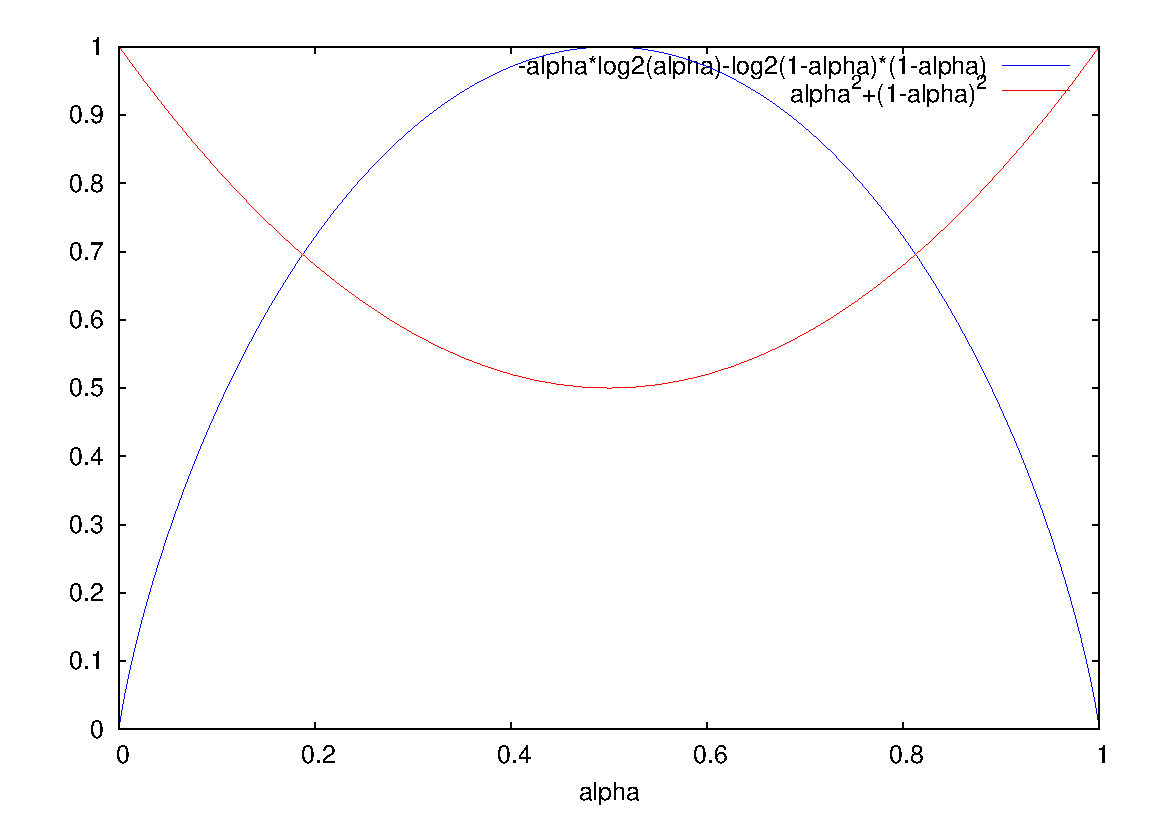
\includegraphics[width=.5\linewidth]{figs/maxout_1}
\end{dmath}
\end{boxedminipage}%
\lthtmlfigureZ
\lthtmlcheckvsize\clearpage}

\stepcounter{section}
\stepcounter{subsection}
\stepcounter{subsection}
\stepcounter{subsection}
\stepcounter{subsection}
\stepcounter{subsection}
\stepcounter{subsection}
\stepcounter{section}
\stepcounter{subsection}
{\newpage\clearpage
\lthtmlinlinemathA{tex2html_wrap_inline2080}%
$C$%
\lthtmlinlinemathZ
\lthtmlcheckvsize\clearpage}

{\newpage\clearpage
\lthtmlinlinemathA{tex2html_wrap_inline2082}%
$D$%
\lthtmlinlinemathZ
\lthtmlcheckvsize\clearpage}

{\newpage\clearpage
\lthtmlinlinemathA{tex2html_wrap_inline2096}%
$16\times16$%
\lthtmlinlinemathZ
\lthtmlcheckvsize\clearpage}

{\newpage\clearpage
\lthtmldisplayA{displaymath2106}%
\begin{displaymath}
{\lvert\alpha \rangle}=\sqrt{\alpha}{\lvert 00 \rangle}+ \sqrt{1-\alpha}{\lvert 11 \rangle},
\end{displaymath}%
\lthtmldisplayZ
\lthtmlcheckvsize\clearpage}

{\newpage\clearpage
\lthtmldisplayA{displaymath2112}%
\begin{displaymath}
{\lvert\beta \rangle}=\sqrt{\beta}{\lvert 00 \rangle}+ \sqrt{1-\beta}{\lvert 11 \rangle},
\end{displaymath}%
\lthtmldisplayZ
\lthtmlcheckvsize\clearpage}

{\newpage\clearpage
\lthtmlinlinemathA{tex2html_wrap_inline2114}%
$\alpha,\beta >1/2$%
\lthtmlinlinemathZ
\lthtmlcheckvsize\clearpage}

{\newpage\clearpage
\lthtmlfigureA{boxedminipage1733}%
\begin{boxedminipage}{2.0\linewidth}
\begin{verbatim}

(%i2) assume(alpha>0,1-alpha>0,beta>0,1-beta>0);
\end{verbatim}

\begin{dmath}[number={\%o2}]
 \left[ \alpha>0,\linebreak[0]\alpha<1,\linebreak[0]\beta>0,\linebreak[0]\beta<1 \right] \end{dmath}
\begin{verbatim}

(%i3) a : schmidt_ket(alpha);
\end{verbatim}

\begin{dmath}[number={\%o3}]
 \pmatrix{\sqrt{\alpha}\cr 0\cr 0\cr \sqrt{1-\alpha}\cr }\end{dmath}
\begin{verbatim}

(%i4) b : schmidt_ket(beta);
\end{verbatim}

\begin{dmath}[number={\%o4}]
 \pmatrix{\sqrt{\beta}\cr 0\cr 0\cr \sqrt{1-\beta}\cr }\end{dmath}
\end{boxedminipage}%
\lthtmlfigureZ
\lthtmlcheckvsize\clearpage}

{\newpage\clearpage
\lthtmlinlinemathA{tex2html_wrap_inline2116}%
$\{E_m\}$%
\lthtmlinlinemathZ
\lthtmlcheckvsize\clearpage}

{\newpage\clearpage
\lthtmlinlinemathA{tex2html_wrap_inline2118}%
$E_m={\lvert u_m \rangle}{\langle u_m \rvert}$%
\lthtmlinlinemathZ
\lthtmlcheckvsize\clearpage}

{\newpage\clearpage
\lthtmlinlinemathA{tex2html_wrap_inline2120}%
$\sum_m E_m=\mathbb{1}_4$%
\lthtmlinlinemathZ
\lthtmlcheckvsize\clearpage}

{\newpage\clearpage
\lthtmlinlinemathA{tex2html_wrap_inline2122}%
$m$%
\lthtmlinlinemathZ
\lthtmlcheckvsize\clearpage}

{\newpage\clearpage
\lthtmlinlinemathA{tex2html_wrap_inline2124}%
${\lvert u_m \rangle}$%
\lthtmlinlinemathZ
\lthtmlcheckvsize\clearpage}

{\newpage\clearpage
\lthtmlfigureA{boxedminipage1751}%
\begin{boxedminipage}{2.0\linewidth}
\begin{verbatim}

(%i5)  declare([u00,u01,u10,u11], complex);
\end{verbatim}

\begin{dmath}[number={\%o5}]
 \mathbf{done}\end{dmath}
\begin{verbatim}

(%i6) u : ket(u00,u01,u10,u11);
\end{verbatim}

\begin{dmath}[number={\%o6}]
 \pmatrix{\mathrm{u00}\cr \mathrm{u01}\cr \mathrm{u10}\cr \mathrm{u11}\cr }\end{dmath}
\end{boxedminipage}%
\lthtmlfigureZ
\lthtmlcheckvsize\clearpage}

{\newpage\clearpage
\lthtmlinlinemathA{tex2html_wrap_inline2126}%
${\lvert\alpha\beta \rangle}{\langle\alpha\beta \rvert}$%
\lthtmlinlinemathZ
\lthtmlcheckvsize\clearpage}

{\newpage\clearpage
\lthtmlinlinemathA{tex2html_wrap_inline2128}%
${\lvert u_m \rangle}{\langle u_m \rvert}$%
\lthtmlinlinemathZ
\lthtmlcheckvsize\clearpage}

{\newpage\clearpage
\lthtmlfigureA{boxedminipage1760}%
\begin{boxedminipage}{2.0\linewidth}
\begin{verbatim}

(%i7) rho : conjsimp((ident(2) otimes toproj(u) otimes ident(2)) . toproj(a otimes b))$,
\end{verbatim}

\end{boxedminipage}%
\lthtmlfigureZ
\lthtmlcheckvsize\clearpage}

{\newpage\clearpage
\lthtmlinlinemathA{tex2html_wrap_inline2134}%
$xx^*$%
\lthtmlinlinemathZ
\lthtmlcheckvsize\clearpage}

{\newpage\clearpage
\lthtmlinlinemathA{tex2html_wrap_inline2136}%
$|x|^2$%
\lthtmlinlinemathZ
\lthtmlcheckvsize\clearpage}

{\newpage\clearpage
\lthtmlinlinemathA{tex2html_wrap_inline2146}%
$2$%
\lthtmlinlinemathZ
\lthtmlcheckvsize\clearpage}

{\newpage\clearpage
\lthtmlinlinemathA{tex2html_wrap_inline2148}%
$3$%
\lthtmlinlinemathZ
\lthtmlcheckvsize\clearpage}

{\newpage\clearpage
\lthtmlinlinemathA{tex2html_wrap_inline2154}%
$\rho_{AD} =\mbox{Tr}_{BC}\rho$%
\lthtmlinlinemathZ
\lthtmlcheckvsize\clearpage}

{\newpage\clearpage
\lthtmlfigureA{boxedminipage1771}%
\begin{boxedminipage}{2.0\linewidth}
\begin{verbatim}

(%i8) rho_14 : ptrace(rho,2,3);
\end{verbatim}

\begin{dmath}[number={\%o8},style={\tiny }]
 \pmatrix{\alpha\*\beta\*\left| \mathrm{u00}\right| ^{2}&\linebreak[0]\alpha\*\sqrt{1-\beta}\*\sqrt{\beta}\*\mathrm{u00}^{\star}\*\mathrm{u01}&\linebreak[0]\sqrt{1-\alpha}\*\sqrt{\alpha}\*\beta\*\mathrm{u00}^{\star}\*\mathrm{u10}&\linebreak[0]\sqrt{1-\alpha}\*\sqrt{\alpha}\*\sqrt{1-\beta}\*\sqrt{\beta}\*\mathrm{u00}^{\star}\*\mathrm{u11}\cr \alpha\*\sqrt{1-\beta}\*\sqrt{\beta}\*\mathrm{u00}\*\mathrm{u01}^{\star}&\linebreak[0]\left(\alpha-\alpha\*\beta\right)\*\left| \mathrm{u01}\right| ^{2}&\linebreak[0]\sqrt{1-\alpha}\*\sqrt{\alpha}\*\sqrt{1-\beta}\*\sqrt{\beta}\*\mathrm{u01}^{\star}\*\mathrm{u10}&\linebreak[0]\left(\sqrt{1-\alpha}\*\sqrt{\alpha}-\sqrt{1-\alpha}\*\sqrt{\alpha}\*\beta\right)\*\mathrm{u01}^{\star}\*\mathrm{u11}\cr \sqrt{1-\alpha}\*\sqrt{\alpha}\*\beta\*\mathrm{u00}\*\mathrm{u10}^{\star}&\linebreak[0]\sqrt{1-\alpha}\*\sqrt{\alpha}\*\sqrt{1-\beta}\*\sqrt{\beta}\*\mathrm{u01}\*\mathrm{u10}^{\star}&\linebreak[0]\left(1-\alpha\right)\*\beta\*\left| \mathrm{u10}\right| ^{2}&\linebreak[0]\left(1-\alpha\right)\*\sqrt{1-\beta}\*\sqrt{\beta}\*\mathrm{u10}^{\star}\*\mathrm{u11}\cr \sqrt{1-\alpha}\*\sqrt{\alpha}\*\sqrt{1-\beta}\*\sqrt{\beta}\*\mathrm{u00}\*\mathrm{u11}^{\star}&\linebreak[0]\left(\sqrt{1-\alpha}\*\sqrt{\alpha}-\sqrt{1-\alpha}\*\sqrt{\alpha}\*\beta\right)\*\mathrm{u01}\*\mathrm{u11}^{\star}&\linebreak[0]\left(1-\alpha\right)\*\sqrt{1-\beta}\*\sqrt{\beta}\*\mathrm{u10}\*\mathrm{u11}^{\star}&\linebreak[0]\left(\left(\alpha-1\right)\*\beta-\alpha+1\right)\*\left| \mathrm{u11}\right| ^{2}\cr }\end{dmath}
\end{boxedminipage}%
\lthtmlfigureZ
\lthtmlcheckvsize\clearpage}

{\newpage\clearpage
\lthtmlinlinemathA{tex2html_wrap_inline2158}%
$\rho_{D} =\mbox{Tr}_{ABC}\rho$%
\lthtmlinlinemathZ
\lthtmlcheckvsize\clearpage}

{\newpage\clearpage
\lthtmlfigureA{boxedminipage1814}%
\begin{boxedminipage}{2.0\linewidth}
\begin{verbatim}

(%i9) rho_4 : ptrace(rho,1,2,3);
\end{verbatim}

\begin{dmath}[number={\%o9}]
 \pmatrix{\left(1-\alpha\right)\*\beta\*\left| \mathrm{u10}\right| ^{2}+\alpha\*\beta\*\left| \mathrm{u00}\right| ^{2}&\linebreak[0]\left(1-\alpha\right)\*\sqrt{1-\beta}\*\sqrt{\beta}\*\mathrm{u10}^{\star}\*\mathrm{u11}+\alpha\*\sqrt{1-\beta}\*\sqrt{\beta}\*\mathrm{u00}^{\star}\*\mathrm{u01}\cr \left(1-\alpha\right)\*\sqrt{1-\beta}\*\sqrt{\beta}\*\mathrm{u10}\*\mathrm{u11}^{\star}+\alpha\*\sqrt{1-\beta}\*\sqrt{\beta}\*\mathrm{u00}\*\mathrm{u01}^{\star}&\linebreak[0]\left(\left(\alpha-1\right)\*\beta-\alpha+1\right)\*\left| \mathrm{u11}\right| ^{2}+\left(\alpha-\alpha\*\beta\right)\*\left| \mathrm{u01}\right| ^{2}\cr }\end{dmath}
\end{boxedminipage}%
\lthtmlfigureZ
\lthtmlcheckvsize\clearpage}

{\newpage\clearpage
\lthtmlinlinemathA{tex2html_wrap_inline2160}%
$\rho_{D}$%
\lthtmlinlinemathZ
\lthtmlcheckvsize\clearpage}

{\newpage\clearpage
\lthtmlinlinemathA{tex2html_wrap_inline2164}%
$M(\mathbb{C},2)$%
\lthtmlinlinemathZ
\lthtmlcheckvsize\clearpage}

{\newpage\clearpage
\lthtmldisplayA{displaymath959}%
\begin{displaymath}
    {\lvert a \rangle}=\sum_{i,j=0}^1 a_{ij}{\lvert ij \rangle}\quad\mapsto\quad\widehat{a}=
    \pmatrix{
      a_{00} & a_{01} \cr
      a_{10} & a_{11} \cr
    },
\end{displaymath}%
\lthtmldisplayZ
\lthtmlcheckvsize\clearpage}

{\newpage\clearpage
\lthtmlinlinemathA{tex2html_wrap_inline2168}%
$X_m^{}X_m^{\dagger}$%
\lthtmlinlinemathZ
\lthtmlcheckvsize\clearpage}

{\newpage\clearpage
\lthtmlinlinemathA{tex2html_wrap_inline2170}%
$X_m = \widehat{\alpha}\,\widehat{u}_m\,\widehat{\beta}$%
\lthtmlinlinemathZ
\lthtmlcheckvsize\clearpage}

{\newpage\clearpage
\lthtmlfigureA{boxedminipage1830}%
\begin{boxedminipage}{2.0\linewidth}
\begin{verbatim}

(%i10) ket_to_mat(iket) := matrix([iket[1,1],iket[2,1]],[iket[3,1],iket[4,1]])$
\end{verbatim}

\end{boxedminipage}%
\lthtmlfigureZ
\lthtmlcheckvsize\clearpage}

{\newpage\clearpage
\lthtmlinlinemathA{tex2html_wrap_inline2172}%
$\rho_D$%
\lthtmlinlinemathZ
\lthtmlcheckvsize\clearpage}

{\newpage\clearpage
\lthtmlfigureA{boxedminipage1835}%
\begin{boxedminipage}{2.0\linewidth}
\begin{verbatim}

(%i11)  X : ket_to_mat(a) . ket_to_mat(u) . ket_to_mat(b);
\end{verbatim}

\begin{dmath}[number={\%o11}]
  \pmatrix{\sqrt{\alpha}\*\sqrt{\beta}\*\mathrm{u00}&\linebreak[0]\sqrt{\alpha}\*\sqrt{1-\beta}\*\mathrm{u01}\cr
    \sqrt{1-\alpha}\*\sqrt{\beta}\*\mathrm{u10}&\linebreak[0]\sqrt{1-\alpha}\*\sqrt{1-\beta}\*\mathrm{u11}\cr
  }\end{dmath} 
\begin{verbatim}

(%i12) rho_4a : conjsimp(ctranspose(X) . X);
\end{verbatim}

\begin{dmath}[number={\%o12}]
 \pmatrix{\left(1-\alpha\right)\*\beta\*\left| \mathrm{u10}\right| ^{2}+\alpha\*\beta\*\left| \mathrm{u00}\right| ^{2}&\linebreak[0]\left(1-\alpha\right)\*\sqrt{1-\beta}\*\sqrt{\beta}\*\mathrm{u10}^{\star}\*\mathrm{u11}+\alpha\*\sqrt{1-\beta}\*\sqrt{\beta}\*\mathrm{u00}^{\star}\*\mathrm{u01}\cr \left(1-\alpha\right)\*\sqrt{1-\beta}\*\sqrt{\beta}\*\mathrm{u10}\*\mathrm{u11}^{\star}+\alpha\*\sqrt{1-\beta}\*\sqrt{\beta}\*\mathrm{u00}\*\mathrm{u01}^{\star}&\linebreak[0]\left(\left(\alpha-1\right)\*\beta-\alpha+1\right)\*\left| \mathrm{u11}\right| ^{2}+\left(\alpha-\alpha\*\beta\right)\*\left| \mathrm{u01}\right| ^{2}\cr }\end{dmath}
\end{boxedminipage}%
\lthtmlfigureZ
\lthtmlcheckvsize\clearpage}

{\newpage\clearpage
\lthtmlinlinemathA{tex2html_wrap_inline2176}%
$p_m=\mbox{Tr}(\rho)=\mbox{Tr}(\rho_D)$%
\lthtmlinlinemathZ
\lthtmlcheckvsize\clearpage}

{\newpage\clearpage
\lthtmlfigureA{boxedminipage1861}%
\begin{boxedminipage}{2.0\linewidth}
\begin{verbatim}

(%i13)  res1 : conjsimp(mat_trace(rho));
\end{verbatim}

\begin{dmath}[number={\%o13}]
 \left(\left(\alpha-1\right)\*\beta-\alpha+1\right)\*\left| \mathrm{u11}\right| ^{2}+\left(1-\alpha\right)\*\beta\*\left| \mathrm{u10}\right| ^{2}+\left(\alpha-\alpha\*\beta\right)\*\left| \mathrm{u01}\right| ^{2}+\alpha\*\beta\*\left| \mathrm{u00}\right| ^{2}\end{dmath}
\begin{verbatim}

(%i14) res2 : conjsimp(mat_trace(rho_4a));
\end{verbatim}

\begin{dmath}[number={\%o14}]
 \left(\left(\alpha-1\right)\*\beta-\alpha+1\right)\*\left| \mathrm{u11}\right| ^{2}+\left(1-\alpha\right)\*\beta\*\left| \mathrm{u10}\right| ^{2}+\left(\alpha-\alpha\*\beta\right)\*\left| \mathrm{u01}\right| ^{2}+\alpha\*\beta\*\left| \mathrm{u00}\right| ^{2}\end{dmath}
\end{boxedminipage}%
\lthtmlfigureZ
\lthtmlcheckvsize\clearpage}

{\newpage\clearpage
\lthtmldisplayA{displaymath1063}%
\begin{displaymath}
 p_m=\sum^1_{i,j=0} \widehat{\alpha}_{i,j}^2 \widehat{\beta}_{i,j}^2 |\widehat{u}_m,ij|^2
\end{displaymath}%
\lthtmldisplayZ
\lthtmlcheckvsize\clearpage}

{\newpage\clearpage
\lthtmlfigureA{boxedminipage1866}%
\begin{boxedminipage}{2.0\linewidth}
\begin{verbatim}

(%i15) res3 : ratsimp(braz(0,0).a^2 * braz(0,0).b^2 *abs(u00)^2+ braz(0,0).a^2 * braz(1,1).b^2 * abs(u01)^2 
    +  braz(1,1).a^2 * braz(0,0).b^2 * abs(u10)^2 +  braz(1,1).a^2 * braz(1,1).b^2 * abs(u11)^2);\end{verbatim}

\begin{dmath}[number={\%o15}]
 \left(\left(\alpha-1\right)\*\beta-\alpha+1\right)\*\left| \mathrm{u11}\right| ^{2}+\left(1-\alpha\right)\*\beta\*\left| \mathrm{u10}\right| ^{2}+\left(\alpha-\alpha\*\beta\right)\*\left| \mathrm{u01}\right| ^{2}+\alpha\*\beta\*\left| \mathrm{u00}\right| ^{2}\end{dmath}
and see that $p_m$\  is the same as above--- verifying this last formula was well. 
\end{boxedminipage}%
\lthtmlfigureZ
\lthtmlcheckvsize\clearpage}


\end{document}
